\documentclass[a4paper,12pt]{book}
\usepackage{graphicx}
\usepackage{tabularx}
\usepackage{a4wide}
%\usepackage[bookmarks=false,breaklinks=true,pdfstartview=Fit]{hyperref}
\usepackage{amsfonts}
\usepackage{amsmath}
%\usepackage{listings}
% \usepackage{color}
\usepackage[usenames,dvipsnames]{color}
\usepackage{html}
%\usepackage{hyperref}
\usepackage{verbatim}
\usepackage{pytex}

% \#c4ebff;

\begin{htmlonly}
\newcounter{pytexcount}
\newcounter{pytexsubcount}
\newcounter{pytexlinecountstart}
\newcounter{pytexlinecountend}

\setcounter{pytexcount}{0}
\setcounter{pytexlinecountstart}{0}
\setcounter{pytexlinecountend}{0}

% Assign a new header
\newenvironment{pytexTemplate}[1]{
\begin{rawhtml}
<div style="display:none">
\end{rawhtml}
}{
\begin{rawhtml}
</div>
\end{rawhtml}
}

\newcommand{\pytexStart}[1]{
  \addtocounter{pytexcount}{1}%   pytexcoun++
  \setcounter{pytexsubcount}{0}%  reset pytexsubcount
}

\renewenvironment{pytex}
{\addtocounter{pytexsubcount}{1}%                                             pytexsubcount++
  %                                                                            each line is added to accumulator
\begin{rawhtml}
<div style="color: black; background-color: \#b9c8db;  border-style: dotted; border-width: 1px; padding:2px;padding-left:1em" >
<pre>
\end{rawhtml}
}%
{\begin{rawhtml}
</pre>
</div>
<div style="color: black; background-color: \#fffff;  border-style: solid; border-width: 1px; padding:2px;padding-left:1em;margin-left:1em;" >\end{rawhtml}
\verbatiminput{pytex_\alph{pytexcount}_\arabic{pytexsubcount}.log}%
\begin{rawhtml}
</div>
\end{rawhtml}
}
\renewenvironment{pytexoutput}
{\addtocounter{pytexsubcount}{1}%                                             pytexsubcount++
  %                                                                            each line is added to accumulator
\begin{rawhtml}
<div style="display:none">
<pre>
\end{rawhtml}
}%
{\begin{rawhtml}
</pre>
</div>
<div style="color: black; background-color: \#fffff;  border-style: solid; border-width: 1px; padding:2px;padding-left:1em;margin-left:1em;" >\end{rawhtml}
\verbatiminput{pytex_\alph{pytexcount}_\arabic{pytexsubcount}.log}%
\begin{rawhtml}
</div>
\end{rawhtml}
}
\newcommand{\codebegin}{
\begin{rawhtml}
<div style="color: black; background-color: \#b9c8db;  border-style: dotted; border-width: 1px;padding:2px;padding-left:1em" >
\end{rawhtml}
}
\newcommand{\codeend}{
\begin{rawhtml}
</div>
\end{rawhtml}
}
\end{htmlonly}

%begin{latexonly}
\newcommand{\codebegin}{

}
\newcommand{\codeend}{

}
%end{latexonly}

\author{Joel Andersson \and Attila Kozma \and Joris Gillis \and Moritz Diehl}
\title{CasADi Users' Guide {\color{red}(WORKING COPY)}}
\begin{document}
%\htmlinfo*
%\sffamily
\titlepage
\maketitle
%\clearpage
\begin{latexonly}
\tableofcontents
\end{latexonly}
\clearpage

\chapter{Introduction}
{\color{red}Warning: The users' guide is not finished. This is only a working copy.}
This document gives a brief tutorial on the CasADi software package and on the interfaces that comes with it. We aim at
introducing the most important capabilities of what CasADi can do. Our fundamental motivation is to provide open-source
software for people working with numerical optimization, dynamic system simulation and optimal control.

Our explaination is mostly program code driven and provides little mathematical background knowledge. We assume that the reader already has a fair knowledge of either Python or C++, theory of differential equations and optimization theory. We will mainly use Python syntax in the discussion, which is the language we recommend using for getting familiar with CasADi, and try to point out the instances where the C++ or Octave syntax diverges from the Python syntax. To facilitate switching between the programming languages, we also list the major differences in Chapter \ref{sec:syntax_differences}. The goal of this document is to make the reader familiar with the syntax of CasADi and provide easily available building blocks to build numerical optimization and dynamic optimization software.

After reading this users' guide, the reader should be able to formulate and manipulate symbolic expressions in CasADi, generate derivatives using algorithmic differentiation, to set up, solve and perform forward and adjoint sensitivity analysis for systems of ordinary differential equations (ODE) or differential-algebraic equations (DAE) as well as to solve nonlinear programming (NLP) problems and optimal control (OCP) problems.

\chapter{Installation}
{\color{red}Warning: This chapter is not up-to-date.}
In this section we introduce step by step the installation procedure of CasADi. First we detail what software packages need to
be installed in order to use CasADi.
\section{Software requirements}
CasADi consists of a symbolic core, which is strongly used by the interfaces that are shipped with it. Now we summarize
what the dependencies of each are. As a general rule you will always need a C++ compiler (tested with gcc 4.4.3) and
CMake (tested with version 2.8.2).
\begin{center}
\small
\begin{tabular}{|l|l|}
\hline
\textbf{Package/interface} & \textbf{Dependency}\\
\hline
CasADi core & None \\
\hline
CSparse interface & CSparse (comes with CasADi)\\
\hline
Ipopt interface & Ipopt\\
\hline
KNITRO interface & KNITRO\\
\hline
LAPACK interface & library with LAPACK api\\
\hline
WORHP interface & WORHP\\
\hline
Sundials interface & SUNDIALS \\
\hline
CasADi for python & SWIG \\
\hline
\end{tabular}
\end{center}
\section{Compilation}
First, you have to get CasADi from \htmladdnormallink{here}{http://www.casadi.org/} or check out the git repository from GitHub.
\par
\codebegin
\begin{verbatim}
git clone https://github.com/casadi/casadi.git -b tested casadi
\end{verbatim}
\codeend
Set the \texttt{CMAKE\_PREFIX\_PATH} to inform CMake where the dependecies are. 
For example if Sundials headers and libraries are installed under \texttt{\$HOME/local/}, then type
\par
\codebegin{
\begin{verbatim}
export CMAKE_PREFIX_PATH=$HOME/local/
\end{verbatim}
\codeend
\par
Go to directory of the source tree, create a directory called \texttt{build} where all compilation-related files will be created.
\par
\codebegin
\begin{verbatim}
cd casadi; mkdir build; cd build
\end{verbatim}
\codeend
Generate the \texttt{Makefile} by typing
\par
\codebegin
\begin{verbatim}
cmake ..
\end{verbatim}
\codeend
Check the output of CMake if the dependencies are correctly located. The interfaces without underlying libraries and headers won't be compiled.
Now compile the C++ libraries.
\par
\codebegin
\begin{verbatim}
make
\end{verbatim}
\codeend
If you wish to use the python interface you can compile it with the \texttt{python} target and install it with the \texttt{install\_python} target.
\par
\codebegin
\begin{verbatim}
make python && sudo make install_python
\end{verbatim}
\codeend

\chapter{Structure of CasADi}
In CasADi a powerful symbolic abstraction of mathematical functions is implemented.
In this chapter we will learn how to create general functions out of our model equations, 
how to evaluate them and optionally their derivatives. We also give some instructional
examples to make it more easily understandable.

The backbone of CasADi is centered around some fundamental classes:
\begin{itemize}
 \item \texttt{SX} -- \emph{scalar symbolic type}
 \item \texttt{SXMatrix} -- \emph{sparse matrix with elements of type \texttt{SX}}
 \item \texttt{DMatrix}  -- \emph{same as \texttt{SXMatrix} but with elements of floating point type}
 \item \texttt{FX} and derived classes -- \emph{functions}
 \item \texttt{MX} -- \emph{matrix symbolic type}
\end{itemize}

\section{\texttt{SX} and \texttt{SXMatrix}}
The \texttt{SX} type is used to represent symbolic expressions made up by a sequence of unary and binary operations. It uses a syntax similar to a numeric type such as \texttt{float} in Python or a \texttt{double} in C/C++, but instead of calculating the expressions numerically, the \texttt{SX} will build up an expression. The type overloads most common operations and can also be used instead of container classes such as \texttt{numpy.array} in Python or \texttt{std::vector<>} in C++'s Standard Template Library (STL).

Though it is possible and somtimes benificial, we shall not work with the \texttt{SX} type directly in this tutorial. Instead we shall work with a \emph{sparse matrix type} called \texttt{SXMatrix}, whose elements are \texttt{SX} instances. \texttt{SXMatrix} uses an everything-is-a-matrix type syntax that should be familiar to Matlab users, which means that scalars can be represented as 1-by-1 matrices and vectors as $n$-by-1 matrices. To store its element, it uses a general sparse matrix format comparible to that used for sparse matrices in Matlab\footnote{To be more precise, the storage format used is \emph{compressed row storage}}.

To see how it works in practice, start an interactive Python shell (e.g. by typing \texttt{ipython} from a Linux terminal or inside a integrated development environment such as Spyder) and import CasADi using the command:\footnote{In C++, include the core header files through ''\texttt{\#include "symbolic/casadi.hpp"}''. Classes and functions are defined in the namespace \texttt{CasADi}. In Octave, the CasADi module is imported by simply invoking \texttt{casadi}}

\begin{pytexTemplate}{main}
from casadi import *
\end{pytexTemplate}

\pytexStart{empty}

\begin{pytex}
from casadi import *
\end{pytex}

Now create the variable \texttt{x} using the syntax (cf. the function \texttt{sym} in Matlab's Symbolic Toolbox)\footnote{In C++, since it is statically typed, you need to specify the return type, here \texttt{SXMatrix}. To find the return types for a CasADi function, use the C++ API docs on the website}:

\begin{pytex}
x = ssym("x")
\end{pytex}

Note that the string passed is only the display name, not the identifier. Multiple variables can have the same name, but still be different. You can also create vectors or matrices of variables using by supplying additional arguments to \texttt{ssym}:
\begin{pytex}
y = ssym("y",5)   # A 5-by-1 matrix, i.e. a vector, with symbolic variables
Z = ssym("Z",4,2) # A 4-by-2 matrix with symbolic variables
\end{pytex}

Note that \texttt{ssym} is a function which returns an \texttt{SXMatrix} instance. When variables have been declared, expressions can now be formed in an intuitive way:
\begin{pytex}
f = x**2 + 10  # "x**y" corresponds to "pow(x,y)" in C++
f = sqrt(f)
print "f = ", f
\end{pytex}

You can also create \texttt{SXMatrix} instances \emph{without} any symbolic variables\footnote{In C++, class}:
\begin{pytex} 
B1 = SXMatrix.zeros(4,5)  # a dense 4-by-5 empty matrix with all zeros
B2 = SXMatrix.sparse(4,5) # a sparse 4-by-5 empty matrix with all zeros
B3 = SXMatrix.ones(4,5)   # a dense 4-by-5 matrix filled with ones
B4 = SXMatrix.eye(4)      # a sparse 4-by-4 matrix with ones on the diagonal
\end{pytex}

Note the difference between a sparse matrix with \emph{structural} zeros and a dense matrix with \emph{actual} zeros. When printing an expression with structural zeros, these will be represented as $00$ to distinguish them from actual zeros $0$.

Elements are accessed and set using a bracket syntax, which also updates the sparsity pattern. Note that in C++ and Python (and thus also in CasADi) indices start with zero:
\begin{pytex} 
print B1[0,0]   # print elements [0,0] (Python is zero-based!)
print B2[-1,-1] # print the last element of the last row
print B3[:,2]   # print all elements in the 3rd column
B4[2:4,1]=[7,3] # set [2,1] to 7 and [3,1] to 3
print B4
\end{pytex}

Remember to pass two arguments if you wish to access a matrix entry. If you call the same function using \emph{one} index, is interpreted as accesssing the (structural) nonzeros of the matrix:
\begin{verbatim}
 B4[:] = 5   # set all nonzeros to 5
 print B4[6] # error: there are only six nonzeros!
\end{verbatim}

There is a growing set of operations that can be performed with the \texttt{SXMatrix}, including:
\begin{itemize}
 \item Calculus: E.g. \verb|Jx = jacobian(f,x)|: Jacobian of expression \texttt{f} with respect to expression \texttt{x}, see also the \texttt{FX} member \emph{function} \texttt{jacobian} below.
 \item Algebra: E.g. \verb|x = solve(A,b)|: Can be used to give a symbolic expression for $x = A^{-1} \, b$.
\end{itemize}
It is typically uncomplicated to add new such functions whenever they appear in applications.

\section{\texttt{DMatrix}}
\texttt{DMatrix} is very similar to \texttt{SXMatrix} (in fact, they are just two template instantiations of the same C++ class \texttt{CasADi::Matrix<\,T\,>}), but with the difference that the nonzero elements are numerical values and not \texttt{SX} expressions. The syntax is also the same, except for functions such as \texttt{ssym} or \texttt{jacobian} which has no equivalent.

\texttt{DMatrix} is mainly used for storing matrices in CasADi and as inputs and outputs of functions. It is \emph{not} intended to be used for computationally intensive calculations. For this purpose, use \texttt{numpy} or \texttt{scipy} matrices in Python or an expression template based library such as \texttt{eigen}, \texttt{ublas} or \texttt{MTL} in C++. Conversion between the types is usually straightforward:
\begin{verbatim}
 C = 4*DMatrix.ones(2,3)
 C[:,2] = 5

 import numpy as NP
 C_numpy = NP.array(C)

 import scipy as SP
 C_scipy = SP.sparse.csr_matrix(C)
\end{verbatim}

More usage examples for \texttt{SX} can be found in the tutorials at \texttt{casadi.org}. For documentation of particular functions of this class (and others), find the ``C++ API docs'' on the website and search for information about \texttt{CasADi::Matrix<\,T\,>}.

\section{\texttt{FX} and derived classes} \label{sec:fx}
CasADi contains a number of functions that all derive from the \texttt{FX} base class. This includes functions that are defined by a symbolic expression, ODE/DAE integrators, QP solvers, NLP solvers etc.

The basic usage skeleton of all these functions are:
\begin{verbatim}
# Call the constructor
f = ClassName(arguments)

# Set options
f.setOption("option_name",option_value)

# Initialize the function
f.init()

# Set inputs, forward and adjoint derivative seeds
f.setInput(value,input_index)

# Evaluate
f.evaluate()

# Get outputs, forward and adjoint derivative sensitivities
f.getOutput(value,output_index)
\end{verbatim}

In Section \ref{sec:ad_numeric}, we extend this skeleton to also includes derivatives.

As an alternative to calling \texttt{getOutput} etc., you can also directly access the internal matrices (which are of type \texttt{DMatrix}). This can decrease overhead and shorten the code, but must be used with caution, since changing the \emph{structure} of these matrices can cause CasADi to crash.
\begin{verbatim}
print "output is ", f.output()
\end{verbatim}

Note that all functions are multiple (sparse, matrix-valued) input, multiple (sparse, matrix-valued) output.

One of the \texttt{FX} derived classes is \texttt{SXFunction}, which defines a function given a symbolic expression. Its constructor is:
\begin{verbatim}
 f = SXFunction(list_of_inputs,list_of_outputs)
\end{verbatim}

There is no mechanism to distinguish the nature of \texttt{FX} functions. For example, any \texttt{FX} with \texttt{DAE\_NUM\_IN} inputs and \texttt{DAE\_NUM\_OUT} outputs can be cosidered to represent a dae function. The CasADi used to generate this documentation has:
\begin{pytexoutput}
print "DAE_NUM_IN = ", DAE_NUM_IN
print "DAE_NUM_OUT = ", DAE_NUM_OUT
\end{pytexoutput}
There are a couple of global constants starting with \texttt{DAE\_} that together constitute the \emph{input/output scheme} of a dae. You can look these up in the API documentation or the python docstrings. You should use these constants and not replace them by the numerical values they happen to have in your version of CasADi, as they might change in the future.\\

For example, here is an excerpt from the documentation for the constructor of a \texttt{CVodesIntegrator}:
\begin{pytexoutput}
docs = CVodesIntegrator.__init__.__doc__.split("\n")
start = docs.index(filter(lambda x: "DAEOutput" in x,docs)[0])
print "\n".join(docs[start:start+4+2*DAE_NUM_OUT])
\end{pytexoutput}

Helper functions are available to construct lists of objects that adhere to a particular scheme. For example, to create a list of a \texttt{DAEOutput} scheme, you use \texttt{daeOut}:

\begin{pytex}
print daeOut()
print daeOut(ode=ssym("fx"))
print daeOut(alg=ssym("fz"),ode=ssym("fx"))
\end{pytex}

Consult the python docstrings for more information of how to use these helper functions:
\begin{pytexoutput}
print daeOut.__doc__
\end{pytexoutput}

All derived classes of \texttt{FX} come with a range of options that can be set. The API documentation shows the list of available options, along with their default values and descriptions. For example, here is an excerpt from the documentation for \texttt{SXFunction}:

\begin{pytexoutput}
docs = SXFunction.__doc__.split("\n")
start = docs.index(filter(lambda x: "List of available options" in x,docs)[0])
print "\n".join(docs[start:start+50])
print "..."
\end{pytexoutput}

You can also query such a list from any object:
\begin{pytex}
x = ssym("x")
f = SXFunction([x],[x])
f.init()
f.printOptions()
\end{pytex}

\begin{pytexoutput}
docs = SXFunction.__doc__.split("\n")
start = docs.index(filter(lambda x: "List of available options" in x,docs)[0])
print "\n".join(docs[start:start+15])
print "..."
\end{pytexoutput}

Two options commonly used during debugging, are "verbose" (a boolean) and "monitor".
The latter allows to specify a list of keywords that each trigger some numerical output to be dumped to the screen when the function is evaluated. A classic example to monitor the objective and constraint function values during NLP solution is as follows:
\begin{verbatim}
solver.setOption("monitor",["eval_f","eval_g"])
\end{verbatim}

Again check the API documentation for details. For example, here is an excerpt from the documentation for of \texttt{IpoptSolver}:
\begin{pytexoutput}
docs = IpoptSolver.__doc__.split("\n")
start = docs.index(filter(lambda x: "List of available monitors" in x,docs)[0])
print "\n".join(docs[start:start+15])
print "..."
\end{pytexoutput}

\section{The \texttt{MX} symbolics}

\pytexStart{main}

Let us perform a simple operation using the \texttt{SXMatrix} above:
\begin{pytex}
x = ssym("x",2,2)
y = ssym("y")
f = 3*x + y
print "f = ", f
\end{pytex}

As you can see, the output of this operaton is a 2-by-2 matrix.

Note how the multiplication and the addition were performed elementwise and new expressions (of type $SX$) were created for each entry of the result matrix.

We shall now introduce a second, more general \emph{matrix expression} type \texttt{MX}. The \texttt{MX} type allows, like \texttt{SX}, to build up expressions consisting of a sequence of elementary operations. But unlike \texttt{SX}, these elementary operations are not restricted to be scalar unary or binary operations ($\mathbb{R} \rightarrow \mathbb{R}$ or $\mathbb{R} \times \mathbb{R} \rightarrow \mathbb{R}$. Instead the elementary operations that are used to form \texttt{MX} expressions are allowed to be general \emph{multiple sparse-matrix valued} input, \emph{multiple sparse-matrix valued} output functions: $\mathbb{R}^{n_1 \times m_1} \times \ldots \times \mathbb{R}^{n_N \times m_N} \rightarrow \mathbb{R}^{p_1 \times q_1} \times \ldots \times \mathbb{R}^{p_M \times q_M}$. In particular, we allow \emph{calls} to functions of type \texttt{FX} (including calls to ODE integrators and \texttt{SXFunction} instances).

The syntax of \texttt{MX} is intended to mirror that of \texttt{SXMatrix}:
\begin{pytex}
x = msym("x",2,2)
y = msym("y")
f = 3*x + y
print "f = ", f
\end{pytex}

where \texttt{msym} has replaced \texttt{ssym}.

Note that this operation required only 2 elementary operations (one multiplication and one addition) using \texttt{MX} symbolics, whereas the \texttt{SX} symbolics required 8 (2 for each element of the resulting matrix). \texttt{MX} is thus more economical when working with operations that are naturally vector or matrix valued. It is also much more general since we allow calls to arbitrary functions that cannot be expanded in terms of elementary operations (like a call to CVodes). %This extra generality, however, comes to the price of more overhead, and we shall 

\texttt{MX} supports getting and setting elements, using the same syntax as \texttt{SXMatrix}, but the way it is implemented is very different. Test, for example, to print the first column of a 2-by-2 symbolic variable:
\begin{pytex}
x = msym("x",2,2)
print x[:,0] 
\end{pytex}

The output should be understood as a (linear) mapping from nonzeros 0 and 2 of the expression \texttt{x} to a new expression of dimension 2-by-1.

Similar outputs can be expected when trying to set elements:
\begin{pytex}
x = msym("x",2)
A = MX.sparse(2,2)
A[0,0] = x[0]
A[1,1] = x[0]+x[1]
print A
\end{pytex}

This time expression \texttt{A} becomes a mapping from \texttt{x} to a sparse 2-by-2 matrix. The interpretation of the cryptic output is that \texttt{A} is a linear mapping from $x$ and $x[0]+x[1]$ onto the diagonal of a (sparse) 2-by-2 matrix. The first nonzero of this mapping is the 0th nonzero of the 0th dependency ($x$) and the second nonzero is the 0th nonzero of the first dependency ($x[0]+x[1]$). 

Linear mappings, of the type you have seen here, is also the the result of several other operations that you might perform on an expression, including (but not limited to) matrix transposes, horizontal and vertical concatenations, resizings and reshapings.

This output tend to become quite hard to understand. An alternative (but not always better) way is to represent the function is as a graph:

\begin{minipage}[t]{0.45\textwidth}
\texttt{from casadi import tools} \\
\texttt{tools.dotdraw(A)} \\
\end{minipage}
\begin{minipage}[t]{0.45\textwidth}
\begin{center}
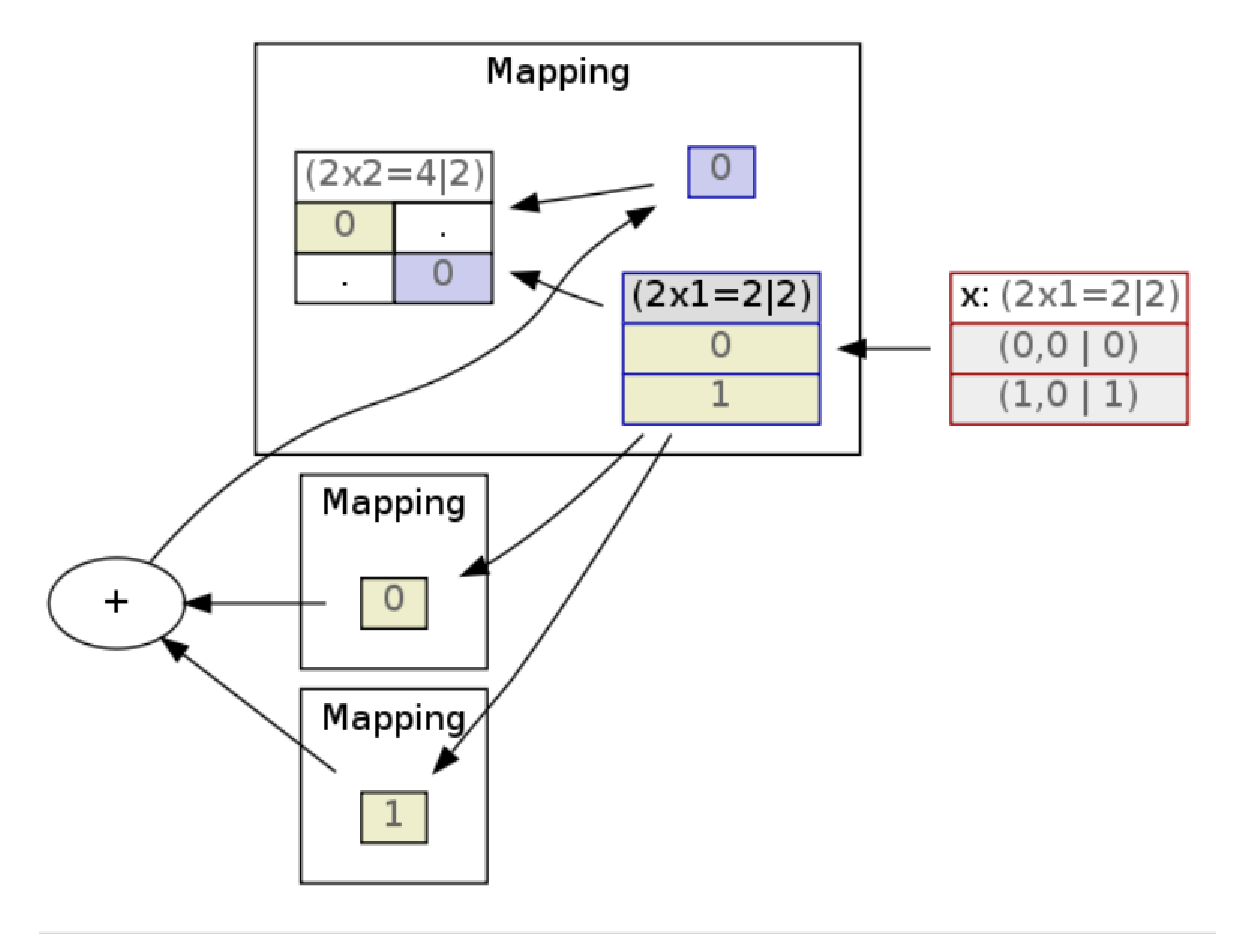
\includegraphics[width=\textwidth]{mxdraw}
\end{center}
\end{minipage}

Using this feature, which is still under development, requires that you have installed the Python package \emph{pydot}. We actively work on getting the expressions more easier to grasp.

\texttt{MX} expressions may contain calls to CasADi functions. To embed a call to an \texttt{FX}-derived function (e.g. \texttt{SXFunction} or \texttt{CVodesIntegrator}, see Section \ref{chapter:integrators}), you use the syntax:
\begin{verbatim}
[y1,y2,...,yn] = f.call([x1,x2,...,xn])
\end{verbatim}

Remember to put the brackets around the output even if the function only has a single output.

Expressions formulated using \texttt{MX} expressions can be used to formulate functions of type \texttt{MXFunction}:
\begin{verbatim}
 f = MXFunction(list_of_inputs,list_of_outputs)
\end{verbatim}

\section{Mixing \texttt{SX} and \texttt{MX}}
You can \emph{not} multiply an \texttt{SXMatrix} with a \texttt{MX}, or perform any other operation to mix the two in the same expression graph. You can, however, as mentioned above, include calls to an \texttt{SXFunction} in an \texttt{MX} graph. This is often a good idea since \texttt{SXFunction} is several times faster than \texttt{MXFunction} when dealing with small to medium size expressions (up to some thousands of variables). It is also much more stable and contains fewer bugs. 

The \texttt{SX} expressions is thus intended to be used for low level operations (for example the DAE right hand side), whereas the \texttt{MX} expressions act as a glue and enables the formulation of e.g. the constraint function of an NLP (which might contain calls to ODE/DAE integrators, or might simply be too large to expand as one big expression).

An \texttt{MXFunction} which only contains built-in operations (e.g. +, *, linear mappings, matrix multiplications and calls to \texttt{SXFunction} instances, can be converted into an \texttt{SXFunction} using the syntax:
\begin{verbatim}
 sx_function = SXFunction(mx_function)
\end{verbatim}

This might speed up the calculations significantly, but might also cause extra memory overhead.

\chapter{Working with CasADi's types}

This chapter aims to give you an in-depth overview of available manipulations on the CasADi primitives, with a focus on the matrix types \texttt{MX} and \texttt{SXMatrix}.

\section{Indexing and slicing}
CasADi offers a variety of different ways to get or set specific elements or blocks of elements in matrix types. Most slicing techniques fall into one of the following two categories:

\begin{description}
\item[nonzero access] aims at non-zeros, specified by their (single) index 
\item[full access] aims at elements in general -- which may well be structural zeros --  specified by a (row, col) pair.
\end{description}

This section gives an exhaustive overview of the possibilities of indexing and slicing. The methods can be used both for setting and getting and they apply to all matrix types: \texttt{MX}, \texttt{SMatrix}, \texttt{DMatrix}, \texttt{IMatrix}.

In python and C++ indexing starts from zero, while in octave indexing starts from 1.
In python, it is customary to use negative indices to specify an index counted from the end of a list. CasADi supports this, too.

\subsection{Getting and setting}

\pytexStart{main}

Each type of slicing comes with a get or set variant.
\begin{pytex}
M = DMatrix([[3,7],[4,5]])
print M[0,:]  # Get variant
M[0,:] = 1    # Set variant
print M
\end{pytex}

Unlike numpy, CasADi slices are not views into the data of the left hand side; rather, a slice access copies the data. As a result, the matrix $M$ is not changed in the following examples: 
\begin{pytex}
M = DMatrix([[3,7],[4,5]])
A = M[0,:]
A.set([1,1])
print A
print M
\end{pytex}

\begin{pytex}
M = DMatrix([[3,7],[4,5]])
M[0,:].set([1,1])
print M
\end{pytex}

\begin{pytex}
M = DMatrix([[3,7],[4,5]])
M[0,:][0,0] = 1 
print M
\end{pytex}

\subsection{Flavours of slices}

\paragraph{Scalar access} is used to target individual elements. The \emph{nonzero access} flavour uses one number, the non-zero index, in rectangular brackets. The \emph{full access} flavour uses two.

An example with a dense matrix:
\begin{pytexoutput}
M = DMatrix([[3,7],[4,5]])

def lprint(s):
  print s,"=", eval(s)
 
def lprints(): 
  lprint("M")
  lprint("M[0]")
  lprint("M[1]")
  lprint("M[2]")
  lprint("M[3]")
  lprint("M[-1]")
  lprint("M[-2]")
  lprint("M[0,0]")
  lprint("M[0,1]")
  lprint("M[1,0]")
  lprint("M[1,1]")
  lprint("M[-1,-1]")
  
lprints()
\end{pytexoutput}

An example with a sparse matrix:
\begin{pytexoutput}
M = diag([3,4,5,6])

lprints()
\end{pytexoutput}

\paragraph{Slice access} is the most common way to access a range of elements at once.
The distinction between \emph{nonzero access} and \emph{full access} is given, again, by the use of either one or two items in the rectangular brackets.
CasADi supports the full range of python slices.

\begin{pytexoutput}
M = DMatrix([[3,7,8,9],[4,5,6,1]])
lprint("M")
lprint("M[:]")    # [3,7,8,9,4,5,6,1]
lprint("M[1:]")   # [  7,8,9,4,5,6,1]
lprint("M[:-1]")  # [3,7,8,9,4,5,6  ]
lprint("M[1:4]")  # [  7,8,9        ]
lprint("M[::3]")  # [3,    9,    6  ]
lprint("M[1,:]")  # [[4,  5,  6,  1 ]]
lprint("M[:,0]")  # [[3],[4]]
lprint("M[0,1]")  # 7
lprint("M[:,1:]") # [[7,8,9],[5,6,1]]
\end{pytexoutput}

\paragraph{List access} are similar to slices in effect, but more flexible.

\begin{pytexoutput}
M = DMatrix([[3,7,8,9],[4,5,6,1]])
lprint("M")
lprint("M[[0,1,2]]")      # [3,7,8]
lprint("M[[6,1,3]]")      # [6,7,9]
lprint("M[0,[0,3]]")      # [[3,  9]]
lprint("M[[1,0],[0,3]]")  # [[4,  1],[3,  9]]
\end{pytexoutput}

\paragraph{Simple IMatrix access} does repeated scalar access with a custom result shape. The user specifies \texttt{IMatrix}'es as item(s) in the rectangular brackets.  The result takes over the shape/sparsity of the supplied \texttt{IMatrix}.

In the \emph{nonzero access} style, each number of the \texttt{IMatrix} supplied is used as non-zero index into the left hand side matrix. In the \emph{full access} style, both \texttt{IMatrix}'es must have the same sparsity. Common non-zeros of the Imatrix'es form (row,col) pairs to access the left hand side.

\begin{pytex}
M = DMatrix([[3,7,8,9],[4,5,6,1]])
k = IMatrix([[0],[1]])
print M[k]    # [[3],[7]]
k = IMatrix([[0,1],[3,6]])
print M[k]    # [[3,  7 ],[9,  6 ]]
k = diag(range(4))
print M[k]    # diag([3,7,8,9])
\end{pytex}

\begin{pytex}
M = DMatrix([[3,7,8,9],[4,5,6,1]])
i = IMatrix([[0],[1]])
j = IMatrix([[2],[3]])
print M[i,j]    # [[8,1]]
i = diag([0,0,1,1])
j = diag([0,1,2,3])
print M[i,j]    # diag([3,7,6,1])
\end{pytex}

\paragraph{Mixed \texttt{IMatrix} access} deals with \emph{nonzero access} in a row or column wise fashion. Given a slice in the rows place and an \texttt{IMatrix} in the columns place, this flavour lets act \emph{simple \texttt{IMatrix} access} on each row individually. The results of all these \emph{simple \texttt{IMatrix} access} are concatenated vertically.

A similar definition holds for an IMatrix in the columns place, and a slice in the rows place of the double element rectangular bracket.

\begin{pytex}
M = DMatrix([[3,7,8,9],[4,5,6,1]])
j = IMatrix([[0],[1]])
print M[0,j]    # [[3],[7]]
print M[1,j]    # [[4],[5]]
print M[:,j]    # [[3],[7],[4],[5]]
\end{pytex}
\begin{pytex}
j = diag([0,2])
print M[:,j]    # [[3,  00 ],[00,  8 ],[4,  00 ],[00,  6 ]]
i = IMatrix([[0,1],[1,0]])
print M[i,:2]   # [[3,  4,  7,  5 ],[4,  3,  5,  7 ]]
\end{pytex}

\paragraph{Sparsity access} involves slicing with a sparsity pattern o fthe same shape as the left hand side. For each non-zero in the slice item, the element of the left hand side with the same (row, col) pair is selected.
\begin{pytex}
M = DMatrix([[3,7,8],[4,5,6],[1,2,9]])
print M[sp_diag(3)]   # diag([3,5,9])
\end{pytex}

\section{Sparsity tools}

Sparsities are easily visualised with the \texttt{spy} command:

\begin{pytex}
sp_diag(3).spy()
\end{pytex}

\subsection{Sparsity constructors}
There are several options to build sparse CasADi matrix types:

\begin{itemize}
 \item Start from an empty matrix and add elements by using indexing/slicing in a setting mode.
 \item Use sparsity contructors
 \item Convert from scipy sparse matrices
\end{itemize}

\begin{pytex}
print DMatrix(sp_tril(3),1)          # [[1,  00,  00 ], [1,  1,  00 ], [1,  1,  1 ]]
print DMatrix(sp_tril(3),range(6))  # [[0,  00,  00 ], [1,  2,  00 ], [3,  4,  5 ]]
\end{pytex}

\paragraph{diagonal}
\begin{pytex}
sp_diag(3).spy()
\end{pytex}

\paragraph{triangular}

\begin{pytex}
sp_tril(3).spy()
\end{pytex}

\paragraph{banded}
\begin{pytex}
sp_band(3,1).spy()
print ""
sp_band(3,-1).spy()
\end{pytex}

\paragraph{row and columsn slices}
\begin{pytex}
sp_rowcol([0,3],[1,2],4,4).spy()
\end{pytex}

\paragraph{(row,col) pairs}
\begin{pytex}
sp_triplet(2,4,[0,1,0,0],[0,1,2,3]).spy()
\end{pytex}

\subsection{Sparsity operators}

The \texttt{+} operator is overloaded for sparsity patterns to perform an \emph{or} operation:

\begin{pytex}
(sp_diag(3)+sp_band(3,1)).spy()
\end{pytex}

The \texttt{*} operator is overloaded for sparsity patterns to perform an \emph{and} operation:

\begin{pytex}
(sp_tril(4)*sp_rowcol([2,3],range(4),4,4)).spy()
\end{pytex}

\chapter{Automatic differentiation\label{chapter:ad}}
The most central functionality of CasADi is \emph{algorithmic (or automatic) differentiation} (AD).

Assume a function $\mathbf{R}^N \rightarrow \mathbf{R}^M$:
\begin{equation}
 y = f(x)
\end{equation}

\emph{Forward mode} directional derivatives can be used to calculate Jacobian-times-vector products:
\begin{equation}
 y_{\text{fsens}} = \frac{\partial f}{\partial x} \, x_{\text{fseed}}
\end{equation}
We will refer to the mulitplying vector as the \emph{seed} vector and the result as the \emph{sensitivity} vector.

Similarily, \emph{adjoint mode} directional derivatives can be used to calculate Jacobian-transposed-times-vector products:
\begin{equation}
 x_{\text{asens}} = \left(\frac{\partial f}{\partial x}\right)^{\text{T}} \, y_{\text{aseed}}
\end{equation}

Both forward and adjoint directional derivatives are calculated at a cost proportinal to evaluating $f(x)$, \emph{regardless of the dimension of $x$}.

CasADi is also able to generate complete, \emph{sparse} Jacobians efficiently. Internally, the algorithm it will use for this depends on the particular \texttt{FX} class but in most cases consists of the following steps:
\begin{itemize}
 \item Automatically detect the sparsity pattern of the Jacobian
 \item Use graph coloring techniques to find a small number of forward and/or directional derivatives needed to construct the complete Jacobian
 \item Calculate the directional derivatives numerically or symbolically
 \item Assemble the complete Jacobian
\end{itemize}

Hessians are calculated by first calcuating the gradient and then performing the same steps as above to calculate the Jacobian of the gradient in the same way as above, while exploiting symmetry.

\section{Calculating directional derivatives numerically} \label{sec:ad_numeric}
Forward and adjoint derivatives can be calculated when a function is numerically evaluated as described in Section \ref{sec:fx}. To achieve this, we extend the usage skeleton as follows:

\begin{verbatim}
# Call the constructor
f = ClassName(arguments)

# Set options
f.setOption("option_name",option_value)

# Initialize the function
f.init()

# Set inputs, forward and adjoint derivative seeds
f.setInput(value,input_index)
f.setFwdSeed(value,input_index)
f.setAdjSeed(value,output_index)

# Evaluate
f.evaluate(num_fwd_sensitivities, num_adj_sensitivities)

# Get outputs, forward and adjoint derivative sensitivities
f.getOutput(value,output_index)
f.getFwdSens(value,output_index)
f.getAdjSens(value,input_index)
\end{verbatim}

Forward and adjoint seeds are set hence together with the function inputs and forward and adjoint sensitivities are collected together with the the function outputs. Multiple forward and/or adjoint derivative directions can be handled simultaneously, that is you can simultaneously multiply the Jacobian from the left or right with multiple vectors.

The number of directional derivatives that be calculated simultaneously is controlled by setting the options \verb|number_of_fwd_dir| and \verb|number_of_adj_dir| (default is 1). If the function is passed as input to another CasADi function (e.g. an ODE integrator or an NLP solver), the number of directional derivatives is allowed to the value set by the options \verb|max_number_of_fwd_dir| and \verb|max_number_of_adj_dir| respectively (default is 64).

\section{Calculating complete Jacobians and Hessians numerically}
You can generate a new function for calculating the Jacobian by calling the \texttt{FX::jacobian} member function:
\begin{verbatim}
 J = f.jacobian(iind,oind) # function corresponding to the jacobian
                           # of the oind-th output w.r.t. the iind-th input
\end{verbatim}
This will generate a function with the same input scheme as the function \texttt{f} but with the (sparse) Jacobian as well as all the original function outputs as outputs.

Similarily, Hessians of a scalar output can be called by calling the \texttt{FX::hessian} member function:
\begin{verbatim}
 H = f.hessian(iind,oind) # function corresponding to the Hessian
                          # of the oind-th output w.r.t. the iind-th input
\end{verbatim}
which will generate a function with the same input scheme as the function \texttt{f} but with the (sparse) Hessian, the gradient and all the original function outputs as outputs.

\section{Calculating derivatives symbolically}
Directional derivatives can also be calculated symbolically, i.e. you can generate new expressions corresponding to directional derivatives for further manipulation. This is only possible for the \texttt{SXFunction} and \texttt{MXFunction} classes.
This is achieved by passing additional arguments to the \texttt{FX::eval} member function.

Similarily, expressions corresponding to complete Jacobians and Hessians can be obtained by calling the \texttt{SXFunction::jac} and \texttt{MXFunction::jac} functions.

We refer to the API documentation for details.

\chapter{ODE/DAE integration and sensitivity analysis} \label{chapter:integrators}
\section{ODE/DAE formulation}
The integrators interfaced with CasADi assumes a DAE residual function of the fully implicit form:
\begin{equation}
 f(t,x,p,\dot{x}) = 0
\end{equation}

Solvers for \emph{ordinary} differential equations will make the additional assumption that the structure of the function is:
\begin{equation}
 f_{\text{ode}}(t,x,p) - \dot{x} = 0
\end{equation}
the explicit equation for $\dot{x}$ can thus be retrieved by simply evaluating the DAE function with $\dot{x} = 0$.

It is important that the arguments of the function uses the order above, and for this reason, we strongly recommend users to work with a set of constants defining the required input and output schemes of the function. For the DAE residual function, these constants are \texttt{DAE\_NUM\_IN=4}, \texttt{DAE\_T=0}, \texttt{DAE\_Y=1}, \texttt{DAE\_P=2} and \texttt{DAE\_YDOT=3} for the inputs and \texttt{DAE\_NUM\_OUT=1} and \texttt{DAE\_RES=0} for the outputs.

An integrator in CasADi is a function that take the state at the initial time, guesses for the algebraic states and state derivatives (only important for DAEs) and evaluates the state vector at the final time. The time horizon is assumed to be fixed\footnote{for problems with free end time, you can always scale time by introducing an extra parameter and substitute $t$ for a dimensionless time variable that goes from 0 to 1} and can be set with the option:
\begin{verbatim}
 integrator.setOption("tf",integration_end_time)
\end{verbatim}

\section{Sundials integrators}
The Sundials suite contains the two popular integrators CVodes and IDAS for ODEs and DAEs respectively. These two integrators supports forward and adjoint sensitivities and when used via CasADi's Sundials interface, CasADi will automatically formulate the Jacobian information, which is needed by the backward differentiation formula (BDF) that CVodes and IDAS use. Also automatically formulated will be the forward and adjoint sensitivitiy equations. This means that the only information that the user needs to provide is the DAE residual function:
\begin{verbatim}
 integrator = CVodesIntegrator(f)   or  integrator = IdasIntegrator(f)
\end{verbatim}
for CVodes and IDAS respectively.

For a list of options for the integrators, as well as the input and output schemes of this \emph{function}, check the documentation directly from Python:
\begin{verbatim}
 CVodesIntegrator?
\end{verbatim}
or by consulting the online C++ API docs on the website.

\section{Sensitivity analysis}
From evaluation point of view, an integrator behaves just like the \texttt{SXFunction} introduced in the previous session. You set inputs, forward/adjoint seeds, evaluate and obtain the outputs and forward/adjoint sensitivities.

\section{The \texttt{Simulator} class}
As already mentioned, integrators in CasADi are functions that calculates the state at the final time. Often, however, a user is interested in obtaining the solution at multiple time points. This can often be done more efficiently than by repeatedly calling \texttt{integrator.evaluate()}. The easiest way to use this functionality is to use the \texttt{Simulator} class.

A \texttt{Simulator} can be created using the syntax:
\begin{verbatim}
  # Import numpy
  import numpy as NP

  # Allocate an integrator instance
  integrator = ...
  integrator.setOption("...",...)

  # Choose a time grid
  tgrid = NP.linspace(0,end_time,num_time_steps)

  # Create a simulator
  simulator = Simulator(integrator, time_grid)
\end{verbatim}

A \texttt{Simulator} can be used just like an integrator, and its input scheme is the same. Its output is now matrix valued, with the the columns corresponding to different time points. The class can also be used to evaluate a particular function of the state at a set of time points. See the API documentation for more information.

% \section{Integration of implicit ODEs}
\chapter{Nonlinear Programming}
The NLP solvers interfaced with CasADi solves parametric NLPs of the following form:
\begin{equation}
\begin{array}{cc}
\begin{array}{c}
\text{minimize:} \\
x \in \mathbb{R}^{nx}, p \in \mathbb{R}^{np}
\end{array}
&
f(x)
\\
\begin{array}{c}
\text{subject to:}
\end{array}
&
\begin{array}{c}
x_{\min} \le x \le x_{\max} \\
g_{\min} \le g(x,p) \le g_{\max}
\end{array}
\end{array}
\end{equation}

With a function \texttt{nlp}, which given $x$ and $p$, gives $f$ and $g$, an NLP solver instance can be allocated by:
\begin{verbatim}
 nlp_solver = IpoptSolver(nlp)
\end{verbatim}

The interface will then automatically generate the information that it might need to solve the NLP, which may be solver and option dependent. Typically an NLP solver will need a function that gives the Jacobian of the constraint function and a Hessian of the Lagrangian function ($L(x,\lambda) = f(x) + \lambda^{\text{T}} \, g(x))$ with respect to $x$. The interface will generate this kind of information automatically and provide to the solver.

NLP solvers, like ODE/DAE integrators are functions in CasADi (though taking derivatives of them is currently not supported). You will find the input and output schemes in the CasADi API documentation on the website or by using the question mark in Python.

\chapter{Optimal control}

\section{Optimal control with CasADi}
CasADi can be used to solve optimal control problem using a variety of methods. As a user, there are two ways to attack the problem:
\begin{itemize}
  \item Use an existing OCP solver
  \item Write your own OCP solver
\end{itemize}

Using an existing OCP solver is attractive for the user who has a relatively simple problem that he wants to test using different methods. In the next exercise, you will get some experience on using such solvers within the JModelica.org framework. Some of these solvers use CasADi.

The option to using an existing solver is to write your own OCP solver. While definitely more involved than using JModelica.org's solver, it is a viable alternative especially when adressing a challenging problem, or a problem using a nonstandard problem formulation. Doing this,   CasADi will take care of things like Jacobian and Hessian generation, sparsity exploitation and all that is left to the user is to perform the reformulation from the infinite dimensional optimal control problem to a finite dimensional NLP.

\section{Optimization of a Van der Pol oscillator}
In CasADi's examples collection, you find codes which all try to solve a simple optimal control problem, a problem borrowed from JModelica.org's examples collection, namely that of driving a \emph{Van der Pol} oscillator to the origin, while trying to minimize a quadratic cost:
\begin{equation}
\begin{array}{lc}
\begin{array}{l}
\text{minimize:} \\
x(\cdot) \in \mathbb{R}^2, \, u(\cdot) \in \mathbb{R}
\end{array}
\quad \displaystyle \int_{t=0}^{10}{(x_0^2 + x_1^2 + u^2) \, dt}
\\
\\
\text{subject to:} \\
\\
\begin{array}{ll}
\left\{
\begin{array}{l}
\dot{x}_0 = (1-x_1^2) \, x_0 - x_1 + u \\
\dot{x}_1 = x_0 \\
-0.75 \le u \le 1.0
\end{array} \right. & \text{for $0 \le t \le 10$} \\
x_0(0)=0, \quad x_0(10)=0  \\
x_1(0)=1, \quad x_1(10)=0  
\end{array}
\end{array}
\label{eq:vdp}
\end{equation}

\section{Direct single-shooting}
The simplest OCP method to implement in CasADi is single-shooting. In fact, it can be implemented in just 30 lines of code, which the script {\texttt{vdp\_single\_shooting.py}} in CasADi's examples collection demonstrates. Please go through the code carefully and make sure that you understand the principle. The most important part of the code are the lines:
\begin{verbatim}
# Build a graph of integrator calls
for k in range(nk):
  [X,Xp] = f_d.call([X,U[k],Xp])
\end{verbatim}

Here, we recursively construct a symbolic expression for the state at the final time. This expression is then used in the formulation of the NLP objective and constraint functions.

\section{Direct multiple-shooting}
The second optimal control method we shall consider is multiple shooting. In multiple shooting, the states at each ''shooting node'' are degrees of freedom in the NLP. The script \\ \texttt{vdp\_multiple\_shooting.py} demonstrates how the VDP problem can be solved using direct multiple shooting in CasADi.

Note how the symbolic variable in the NLP functions now contains both the control and states for each of the \texttt{nk} intervals:
\begin{verbatim}
# Total number of variables
nv = 1*nk + 3*(nk+1)

# Declare variable vector
V = msym("V", nv)
\end{verbatim}

Also note how the recursive overwriting of \texttt{X} has been replaced with:
\begin{verbatim}
for k in range(nk):
  # Local state vector
  Xk = vertcat((X0[k],X1[k],X2[k]))
  Xk_next = vertcat((X0[k+1],X1[k+1],X2[k+1]))
  
  # Call the integrator
  [Xk_end,Xp] = f_d.call([Xk,U[k],Xp])
  
  # append continuity constraints
  g.append(Xk_next - Xk_end)
  g_min.append(NP.zeros(Xk.size()))
  g_max.append(NP.zeros(Xk.size()))
\end{verbatim}

\section{Direct collocation}
When we went from direct single shooting to direct multiple shooting we essentially traded nonlinearity for problem size. The NLP in single shooting is small, but often highly nonlinear, whereas the NLP for multiple-shooting is larger, but less nonlinear.

Direct collocation is to take one more step in the same direction: we achieve an even less nonlinear NLP, at the cost of an even larger NLP.

While multiple shooting only includes the state at the beginning of each control interval as a degree of freedom in the NLP (in addition to the discretized control and the parameters), in direct collocation the state at a set of \emph{collocation points} (in addition to the beginning of the interval) enters in the NLP as variables. An example of a choice of time points are the \emph{Legendre points} of order $d=3$ :
\begin{equation}
 \tau = [0,0.112702,0.500000,0.887298]
\end{equation}

Keeping the same control discretization as in single and multiple shooting:
\begin{equation}
 u(t) = u_k, \quad \text{for $t \in [t_k, t_{k+1}], \quad k=0,\ldots,n_k-1$}
\end{equation}

the complete list of time points, with $h_k := t_{k+1}-t_k$, is:
\begin{equation}
 t_{k,j} := t_k + h_k \, \tau_j, \quad \text{for $k=0,\ldots,n_k-1$ and $j=0,\ldots,d$}
\end{equation}
as well as the final time $t_{n_k,0}$. Also let $x_{k,j}$ denote the states at these time points.

On each control interval, we shall define a Lagrangian polynomial basis:
\begin{equation}
 L_j(\tau) = \prod_{r=0, \, r \ne j}^{d} \frac{\tau - \tau_{r}}{\tau_j - \tau_r}
\end{equation}

Since the Lagrangian basis satisfies:
\begin{equation}
 L_j(\tau_r) = \left\{
 \begin{array}{l}
  1, \qquad \text{if $j=r$} \\
  0, \qquad \text{otherwise}
 \end{array}
  \right.
\end{equation}
we can approximate the state trajectory approximation as a linear combination of these basis functions:
\begin{equation}
\tilde{x}_k(t) = \sum_{r=0}^{d}{L_r\left(\frac{t-t_k}{h_k}\right) \, x_{k,r}}
\end{equation}

In particular we get approximations of the state time derivative at each collocation point (not including $\tau_0$):
\begin{equation}
\tilde{\dot{x}}_k(t_{k,j}) = \frac{1}{h_k} \, \sum_{r=0}^{d}{\dot{L}_r(\tau_j) \, x_{k,r}} := \frac{1}{h_k} \, \sum_{r=0}^{d}{C_{r,j} \, x_{k,r}}
\label{eq:colldef}
\end{equation}

as well as an approximation of the state at the end of the control interval:
\begin{equation}
\tilde{x}_{k+1,0} = \sum_{r=0}^{d}{L_r(1) \, x_{k,r}} := \sum_{r=0}^{d}{D_r \, x_{k,r}}
\label{eq:contdef}
\end{equation}

Plugging in the approximation of the state derivative (\ref{eq:colldef}) into the ODE gives us a set of \emph{collocation equations} that needs to be satisfied for every state at every collocation point:
\begin{equation}
h_k \, f(t_{k,j},x_{k,j},u_k) - \sum_{r=0}^{d}{C_{r,j} \, x_{k,r}} = 0, \qquad k=0,\ldots,n_k-1, \quad j=1,\ldots,d
\end{equation}

And the approximation of the end state (\ref{eq:contdef}) gives us a set of \emph{continuity equations} that must be satisfied for every control interval:
\begin{equation}
x_{k+1,0} - \sum_{r=0}^{d}{D_r \, x_{k,r}} = 0, \qquad k=0,\ldots,n_k-1, 
\end{equation}

These two sets of equations take the place of the continuity equation (represented by the integrator call) in direct multiple shooting. The above equations have been implemented in the script \texttt{vdp\_collocation.py}.

\chapter{Model import from Modelica}\label{sec:modelica}
CasADi contains a facility to import dynamic system models formulated in the Modelica modelling language as well as in the Optimica extension of Modelica to optimal control. The import facility currently works with the open-source \htmladdnormallink{JModelica.org}{http://www.jmodelica.org/} compiler.

For instructions on how to install and use JModelica.org, we refer to their \htmladdnormallink{website}{http://www.jmodelica.org/}. CasADi currently comes bundled with JModelica.org and the JModelica.org trunk is synchronized with CasADi's trunk, simplifying the installation procedure. Pre-built JModelica.org binaries that include CasADi are available for Windows users.

\section{Compiling the Modelica code} \label{sec:modelica_compilation}
To see how to use the Modelica import, look at \htmladdnormallink{thermodynamics\_example.py}{https://github.com/casadi/casadi/blob/tested/examples/python/modelica/fritzson_application_examples/thermodynamics_example.py} and \htmladdnormallink{cstr.cpp}{https://github.com/casadi/casadi/blob/tested/examples/cplusplus/cstr.cpp} in CasADi's example collection. 

Assuming that the Modelica/Optimica model \texttt{ModelicaClass.ModelicaModel} is defined in the files \texttt{file1.mo} and \texttt{file2.mop}, the compile command is:
\begin{verbatim}
  from pymodelica import compile_jmu
  jmu_name=compile_jmu('ModelicaClass.ModelicaModel', \
    ['file1.mo','file2.mop'],'auto','ipopt',\
    {'generate_xml_equations':True, 'generate_fmi_me_xml':False})
\end{verbatim}

This will generate a \texttt{jmu}-file, which is essentially a zipfile containing, among other things, the file \texttt{modelDescription.xml}. This XML-file contains a symbolic representation of the optimal control problem and can be inspected in a standard XML editor.
\begin{verbatim}
  from zipfile import ZipFile
  sfile = ZipFile(jmu_name','r')
  mfile = sfile.extract('modelDescription.xml','.')
\end{verbatim}

\section{The SymbolicOCP class} \label{sec:modelica_import}
The symbolic optimal control problem representation (or just model description) contained in \texttt{modelDescription.xml} can be imported into CasADi in the form of the SymbolicOCP class:
\begin{verbatim}
ocp = SymbolicOCP()
\end{verbatim}

The SymbolicOCP class contains symbolic representation of the optimal control problem designed to be general and allow manipulation. The basic usage of this class is to call the member function \texttt{parseFMI} with the XML file name and a set of options\footnote{In C++, the dictionary with options corresponds to a \texttt{CasADi::Dictionary} object}:
\begin{verbatim}
ocp.parseFMI('modelDescription.xml',{'scale_variables':True})
\end{verbatim}

For a more detailed description of this class and its functionalities, we refer to the API documentation.

\chapter{Syntax differences between CasADi in Python, C++ and Octave}\label{sec:syntax_differences}
\scriptsize
\begin{center}
  \begin{tabular}{| p{3.5cm} | p{3.5cm} | p{3.5cm} | p{3.5cm} | }
    \hline
      & Python & C++ & Octave \\ \hline
    Starting CasADi & \verb|from casadi import *| & \verb|#include \| \verb|"casadi/casadi.hpp"| \verb|using namespace CasADi;| & \verb|casadi| \\ \hline
    Printing the \emph{representation} (string representation intended to be \emph{unambiguous}) & \verb|A <ENTER>| (interactive), \verb|print repr(A)| (in scripts) & \verb|std::cout << A;|& \verb|A <ENTER>| or \verb|disp A|\\ \hline
    Printing the \emph{description} (string representation intended to be \emph{readable}) & \verb|print A| & \verb|A.print();| or \verb|A.print(stream);|& \verb|A.print()| \\ \hline
    Calling a class function & \verb|SXMatrix.zeros(3,4)| & \verb|SXMatrix::zeros(3,4)| & \verb|SXMatrix.zeros(3,4)|\\ \hline
    Reference to a class (e.g. passed to a function as an option) & \verb|ClassName| or \verb|ClassName.creator| & \verb|ClassName::creator| & \verb|ClassName.creator|\\ \hline
    Element access & \verb|A[i,j]|, \emph{0-based} & \verb|A(i,j)| and \verb|A(i)|, \emph{0-based} & \verb|A(i,j)|, \emph{1-based} \\ \hline
    Element assignment & \verb|A[i,j] = b|, \emph{0-based} & \verb|A(i,j) = b| and \verb|A(i) = b|, \linebreak \emph{0-based} & \verb|A(i,j) = b|, \emph{1-based} \\ \hline
    Nonzero access & \verb|A[k]|, \emph{0-based} & \verb|A[k]|, \emph{0-based} & \verb|A(k)|, \emph{1-based} \\ \hline
    Nonzero assignment & \verb|A[k] = b|, \emph{0-based} & \verb|A[k] = b|, \emph{0-based} & \verb|A(k) = b|, \emph{1-based} \\ \hline
    Matrix multiplication & \verb|mul(x,y)| & \verb|mul(x,y)| & \verb|mul(x,y)| or \verb|x*y| \\ \hline
    Elementwise multiplication & \verb|x*y| & \verb|x*y| & \verb|x.*y| \\ \hline
    Elementwise division & \verb|x/y| & \verb|x/y| & \verb|x./y| \\ \hline
    Power & \verb|x**y| & \verb|pow(x,y)| & \verb|x^y| or \verb|x.^y| \\ \hline
    Transpose & \verb|trans(A)| or \verb|A.T| & \verb|trans(A)| & \verb|trans(A)| or \verb|A'| or \verb|A.'| \\ \hline
    Creating a dictionary (e.g. for options) & \verb|d = {'opt1':opt1}| or \verb|d = {}; a['opt1'] = opt1| & \verb|a = Dictionary();| \verb|a['opt1'] = opt1;| & \verb|a = Dictionary();| \verb|a('opt1') = opt1;| (?) \\ \hline
  \end{tabular}
\end{center}

%\bibliographystyle{plain}
%\bibliography{optec}
\end{document}
